\documentclass[12pt]{article}

\usepackage[utf8]{inputenc}
\usepackage[T1]{fontenc}
\usepackage{datetime}
\usepackage[spanish]{babel}
\usepackage{graphicx}
\usepackage{listings}
\usepackage{caption}
\usepackage{subcaption}
\usepackage[right=2cm,left=2cm,top=2cm,bottom=2cm]{geometry}
\usepackage{hyperref}
\usepackage{fancyhdr}
\usepackage{color}
\usepackage[export]{adjustbox}
\usepackage{graphicx}
\usepackage{float}
\usepackage{changepage}
\usepackage{multicol}
\usepackage{imakeidx}
\usepackage{csquotes}
\usepackage{array}
\usepackage{tabularx}
\usepackage{xcolor}
\usepackage[backend=biber]{biblatex}
\addbibresource{webgrafia.bib}

\pagestyle{fancy}
\renewcommand{\footrulewidth}{0.4pt}
\setlength{\headheight}{15pt}


\fancyhead[L]{ CEIABD – BDA }
\fancyhead[R]{Páez Anguita, Víctor }
\fancyfoot[L]{IES Gran Capitán}

\begin{document}

\begin{titlepage}
    \begin{center}
      \Large \bfseries{}
    \end{center}
    \vspace{0.1cm}
    \begin{center}
      \Large \bfseries{}
    \end{center}
    \vspace{0.1cm}
    \begin{center}
     \Large \bfseries{Proyecto final BDA}
    \end{center}
    \vspace{0.0001cm}
    \begin{center}
        Departamento de informática \\ I.E.S. Gran Capitán - Córdoba
    \end{center}
        \vspace{2 cm}
\begin{figure}[h!]
    \centering
    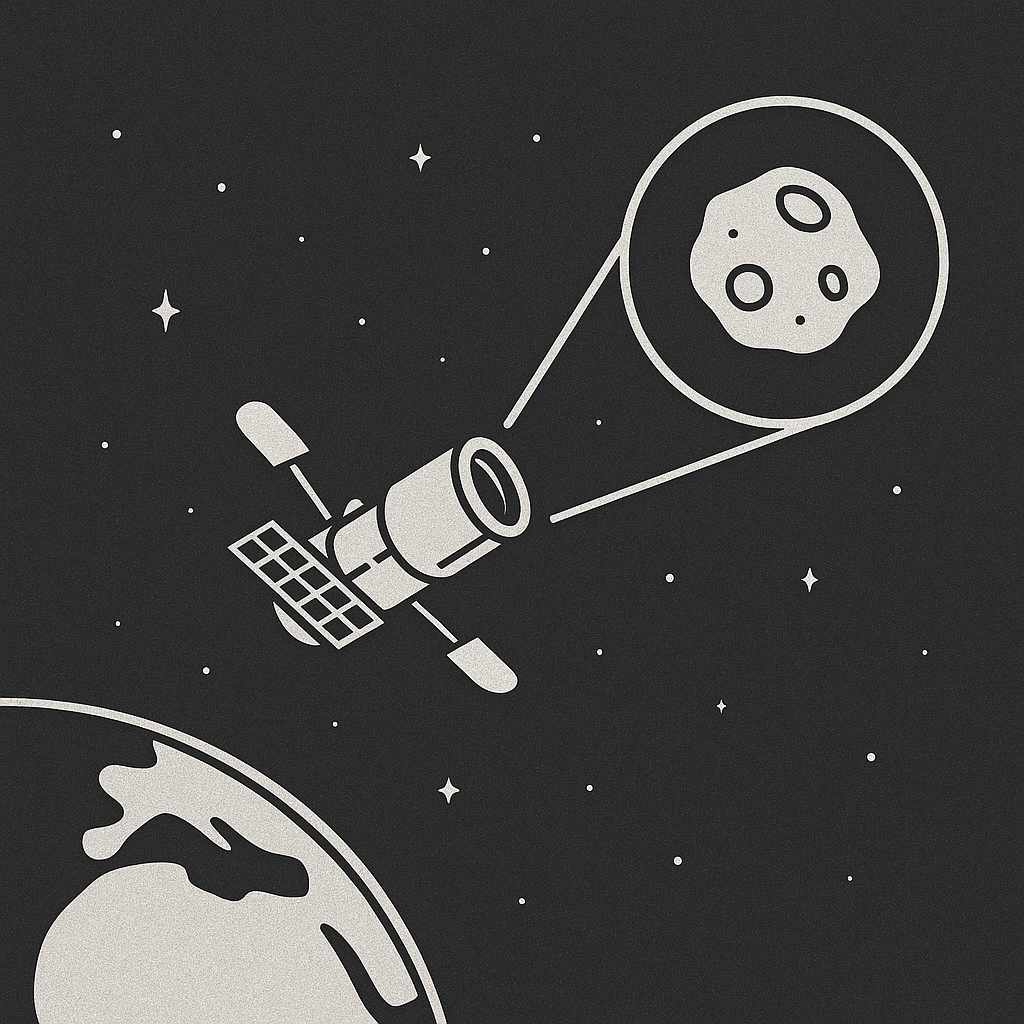
\includegraphics[width=.6\textwidth]{assets/portada.jpg}
    \label{fig:my_label}
\end{figure}
    \vspace{0.2 cm}
    \begin{center}
        Inteligencia artificial y Big data \\ \today 
    \end{center}
    \vspace{4 cm}
\null\hfill \textbf{Desarrollado por:}
\\
\\
\null\hfill Víctor Páez Anguita
\clearpage
\end{titlepage}

%%%%%%%%%%%%%%%%%%%%%%%%%%%Index%%%%%%%%%%%%%%%%%%%%%%%%%%%%%%%%
\tableofcontents
\clearpage
%%%%%%%%%%%%%%%%%%%%%%%%%%%Index%%%%%%%%%%%%%%%%%%%%%%%%%%%%%%%%


\section{Requisitos}

\begin{itemize}
  \item El proyecto deberá tener todo el stack de todos los sistemas vistos en clase perfectamente instalado, configurado y funcionando como un 
  Sistema completo de Big Data, desde la ingesta de datos, ETL, BI y su visualización.

  \item El alumnado elegirá el origen, los tipos y la temática de los datos que se van a procesar en el Sistema Big Data.
  
  \item Deben establecer, desarrollar y justificar el tipo de conocimiento que van a obtener de los datos origen después de su ingesta y 
  procesamiento (ETL) en el sistema.

  \item El procesamiento de los datos lo realizarán a través de SPARK, utilizando alguna de sus 3 APIs disponibles. Esto no quita que puedan 
  realizar algún tipo de procesamiento de datos anteriormente, como por ejemplo en Kafka.

  \item El sistema debe poder soportar la ingesta de datos tanto en batch como en streaming.
  
  \item Los datos de origen podrán ser sintéticos, reales o una combinación de ambos.
  
  \item Puedes usar las Api/s que creas necesaria/s. Incluso la creación de tus propios datos sintéticos en batch y streaming 
  (Estos deben cumplir con los requisitos del puntos 1 al 3)

  \item Todo el ETL realizado deberá estar correctamente desarrollado y justificado.
  
  \item Se deberá añadir al stack algún sistema, servicio, ... de investigación propia 
  (al menos 1, aunque puede añadir todos los que quieras). Se propone una lista de ellos, 
  que podrán ser ampliados a propuesta del alumnado:

  \begin{itemize}
    \item AWS GLUE
    \item AWS S3
    \item Nifi
    \item Flink
    \item Tableau
    \item PowerBI
    \item Elasticsearch
    \item Kibana
    \item RabbitMQ
    \item Otros (deben ser consensuados y aprobados)
  \end{itemize}

  \item La calificación del proyecto se hará de forma global, dependiendo de los niveles de aprendizaje que se demuestres superados acorde 
  al nivel de conocimiento que exige el módulo del CE.
\end{itemize}

\subsection{Proyectos. Requisitos mínimos}
\begin{itemize}
  \item El sistema completo será, como mínimo (más la investigación propia):
  \begin{itemize}
    \item Apache Hadoop Common
    \item HDFS
    \item MapReduce
    \item Yarn
    \item SPARK
    \item Grafana
  \end{itemize}
  \item Debe haber como mínimo 3 nodos en los clusters (en cada uno):
  \begin{itemize}
    \item Hadoop (HDFS/Yarn)
    \item Spark
    \item Kafka
  \end{itemize}
  \item Añade todos los nodos que necesites para desplegar todo el stack Big Data del proyecto.
  \item Deben soportar acceso concurrente desde varios nodos Edge.
\end{itemize}

\subsection{Consideraciones}

\begin{itemize}
  \item A mayor y mejor ETL y mayor y mejor Business Intelligence, mejor calificación.
  \item Si un proyecto no tiene suficiente procesamiento de datos y obtención de conocimiento, 
  mayor será la exigencia de la investigación propia o viceversa.
\end{itemize}

\clearpage

\section{Introducción}

Este proyecto consiste en el desarrollo de un sistema completo de Big Data cuyo objetivo es la detección 
y análisis de objetos cercanos a la Tierra (NEOs, por sus siglas en inglés), como asteroides 
potencialmente peligrosos. A partir de un conjunto de datos base real proporcionado por la NASA 
(Sentry System), se generan datos sintéticos tanto en modo batch como en tiempo real (streaming) 
para simular un flujo continuo de información que pueda ser procesado, transformado y visualizado.
\\
\\
Este proyecto de big data tiene por objetivo la detección y análisis de objectos cercanos a la Tierra
como asteroides, cometas, satelites y otros tipos de objetos que pueden llegar a ser potencialmente
peligrosos. 
\\
Para los datos he utilizado un dataset real de referencia de la NASA el cuál esta en el siguiente
enlace: 
\\
\\
\url{https://cneos.jpl.nasa.gov/sentry/}.
\\
\\
El problema que tenemos es que este dataset al no ser lo suficientemente grande, y Además
de que no contiene datos en tiempo real, he decidido crear un dataset con datos sintéticos,
basado en el dataset anterior y añadiendo algunos datos más. Los datos sintéticos serán 
generados con la librería Faker, que permite crear datos falsos de forma sencilla y rápida.
\\
\\
\url{https://github.com/joke2k/faker}.
\\
\\
De este modo puedo simular un flujo de datos continuo que pueda ser procesado, transformado 
y visualizado.
\\
\\
El sistema implementa todo el stack tecnológico necesario. Teniendo una arquitectura basada en 
un clúster de Apache hadoop desplegado en un entorno distribuido con HDFS, que permite realizar
la ingesta de datos recogeremos los datos con un cluster de kafka que se encargará de recibir
los datos en tiempo real y almacenarlos en un topic. para su posterior procesamiento utilizando
las APIs de Spark Streaming y Spark SQL.
\\
\\
Los datos origen han sido diseñados para incluir valores realistas (como fecha de posible impacto, 
distancia mínima a la Tierra, probabilidad de colisión o tamaño del objeto), junto con datos 
erróneos o incompletos, con el fin de justificar y aplicar transformaciones durante la fase de ETL. 
El conocimiento que se pretende extraer del sistema incluye la identificación y clasificación de 
objetos potencialmente peligrosos, el análisis de tendencias a lo largo del tiempo, y la 
posibilidad de generar alertas en función de parámetros críticos como la proximidad o la 
velocidad del asteroide.
\\
\\
Mediante la integración de Power BI, se realizarán las correspondientes visualizaciones 
a través de los dashboards para facilitar la toma de decisiones y el análisis exploratorio de 
los resultados.

\clearpage

\section{Ingesta de datos}



\clearpage

\section{Conclusión}


\clearpage

\section{Bibliografia}

\cite{Botpress}

\printbibliography

\end{document}
